\documentclass[10pt,a4paper]{article}
% Оформление: ivanshemidko/algebra-notes, s2/main.tex,
% commit d52e89ab46b905aac035e556794af91aec7c86ef.
\usepackage{fontspec}
% Project-local installation keeps local and CI font files identical.
\setmainfont{cmunrm.ttf}[
  Path=fonts/,
  BoldFont=cmunbx.ttf,
  ItalicFont=cmunti.ttf,
  BoldItalicFont=cmunbi.ttf
]
\usepackage[english,russian]{babel}
\usepackage{amsmath,amssymb,mathtools,amsthm}
% Unicode maps for traditional Computer Modern math fonts (search/copy text).
\pdfvariable gentounicode=1
\protected\def\pdfglyphtounicode{\pdfextension glyphtounicode}
\input{glyphtounicode.tex}
% The standard map omits CMEX's sized delimiter glyph names.
\ExplSyntaxOn
\clist_map_inline:nn {big,Big,bigg,Bigg} {
  \pdfglyphtounicode{parenleft#1}{0028}
  \pdfglyphtounicode{parenright#1}{0029}
  \pdfglyphtounicode{braceleft#1}{007B}
  \pdfglyphtounicode{braceright#1}{007D}
  \pdfglyphtounicode{bracketleft#1}{005B}
  \pdfglyphtounicode{bracketright#1}{005D}
  \pdfglyphtounicode{floorleft#1}{230A}
  \pdfglyphtounicode{floorright#1}{230B}
  \pdfglyphtounicode{ceilingleft#1}{2308}
  \pdfglyphtounicode{ceilingright#1}{2309}
  \pdfglyphtounicode{angbracketleft#1}{27E8}
  \pdfglyphtounicode{angbracketright#1}{27E9}
  \pdfglyphtounicode{slash#1}{002F}
  \pdfglyphtounicode{backslash#1}{005C}
}
\ExplSyntaxOff
\usepackage{geometry}
\geometry{left=22mm,right=22mm,top=25mm,bottom=27mm,heightrounded}
\usepackage{enumitem}
\usepackage[most]{tcolorbox}
\tcbuselibrary{theorems,breakable,skins}
\usepackage{graphicx,caption}
\captionsetup{font=small,labelfont=bf,hypcap=false}

\definecolor{cbBlueBack}{RGB}{246,249,252}
\definecolor{cbGreenBack}{RGB}{246,251,248}
\definecolor{cbOrangeBack}{RGB}{252,249,242}
\definecolor{cbPurpleBack}{RGB}{249,247,252}
\definecolor{cbGrayBack}{RGB}{249,249,249}
\definecolor{cbBlue}{RGB}{42,87,132}
\definecolor{cbGreen}{RGB}{52,110,72}
\definecolor{cbOrange}{RGB}{140,98,0}
\definecolor{cbPurple}{RGB}{93,78,140}
\definecolor{cbGray}{RGB}{80,80,80}

\newtheoremstyle{mystatement}{8pt}{8pt}{\itshape}{}{\bfseries}{.}{\newline}{}
\newtheoremstyle{mydefinition}{8pt}{8pt}{\normalfont}{}{\bfseries}{.}{0.5em}{}
\theoremstyle{mystatement}
\newtheorem{theorem}{Теорема}[part]
\newtheorem{lemma}{Лемма}[part]
\newtheorem{cor}{Следствие}[part]
\theoremstyle{mydefinition}
\newtheorem{definition}{Определение}[part]
\newtheorem{example}{Пример}[part]
\numberwithin{equation}{part}
\counterwithin{figure}{part}
\tcbset{
  enhanced,sharp corners,boxrule=0.5pt,
  left=9pt,right=9pt,top=7pt,bottom=7pt,
  before skip=8pt,after skip=8pt,breakable
}
\tcolorboxenvironment{theorem}{colback=cbBlueBack,colframe=cbGray!55,borderline west={1.6pt}{0pt}{cbBlue}}
\tcolorboxenvironment{lemma}{colback=cbBlueBack,colframe=cbGray!55,borderline west={1.6pt}{0pt}{cbBlue}}
\tcolorboxenvironment{cor}{colback=cbPurpleBack,colframe=cbGray!55,borderline west={1.6pt}{0pt}{cbPurple}}
\tcolorboxenvironment{definition}{colback=cbGreenBack,colframe=cbGreen!55!cbGray,borderline west={1.6pt}{0pt}{cbGreen}}
\tcolorboxenvironment{example}{colback=cbOrangeBack,colframe=cbOrange!45!cbGray,borderline west={1.6pt}{0pt}{cbOrange}}

\usepackage{hyperref}
\hypersetup{
  colorlinks=true,linkcolor=cbBlue,citecolor=cbBlue,urlcolor=cbBlue,
  pdftitle={Математический анализ · III семестр},
  pdfauthor={},pdfsubject={},pdfcreator={LuaLaTeX}
}
\linespread{1.0}
\setlength{\parindent}{0pt}
\setlength{\parskip}{4pt}
\allowdisplaybreaks[1]
\providecommand{\tightlist}{\setlength{\itemsep}{0pt}\setlength{\parskip}{0pt}}

\usepackage{titlesec}
\titleformat{\part}[block]{\Large\bfseries\centering}{}{0pt}{}
\titlespacing*{\part}{0pt}{0pt}{12pt}
\counterwithin{section}{part}
\renewcommand{\thepart}{\arabic{part}}
\usepackage{tocloft}
\setlength{\cftsecnumwidth}{2.8em}
\setlength{\cftsubsecnumwidth}{3.6em}
\setcounter{tocdepth}{2}
\usepackage{fancyhdr}
\pagestyle{fancy}
\fancyhf{}
\fancyhead[L]{\nouppercase{\leftmark}}
\fancyfoot[C]{\thepage}
\let\oldpart\part
\renewcommand{\part}[1]{\oldpart{#1}\markboth{#1}{}}
\renewcommand{\sectionmark}[1]{}
\usepackage{etoolbox}
\pretocmd{\part}{\newpage}{}{}

\begin{document}
\thispagestyle{empty}
\begin{center}
  {\LARGE\bfseries Математический анализ · III семестр}
\end{center}
\vspace{12pt}
\tableofcontents

\part{Функциональные последовательности}\label{sec-sequences}
\section{\texorpdfstring{Равномерная сходимость. Пространство \(\ell^\infty(\Omega)\)}{Равномерная сходимость. Пространство ограниченных функций}}\label{sec-sequences-01}

Напоминание: нормированное пространство, полное относительно метрики, порождённой нормой, называется \textbf{банаховым}.

В конечномерном пространстве эквивалентны все \emph{нормы}. В бесконечномерном пространстве нормы могут быть неэквивалентны.

\begin{definition}[Пространство ограниченных функций]\label{def-bounded}

\(\ell^\infty(\Omega)\) --- множество функций \(f:\Omega\to\mathbb C\), ограниченных по модулю: \[
\exists C>0\quad\forall x\in\Omega:\quad |f(x)|\le C.
\] На нём задаётся норма

\begin{equation}
\lVert f\rVert_\infty=\sup_{x\in\Omega}|f(x)|,
\qquad d(f,g)=\lVert f-g\rVert_\infty.
\label{eq-sup-norm}
\end{equation}

Метрика \(d\) называется чебышевским расстоянием.

\end{definition}

\begin{definition}[Равномерная сходимость]\label{def-uniform-sequence}

Последовательность \(\{f_n\}_{n=1}^{\infty}\) равномерно сходится на \(\Omega\) к \(f\), если \[
\lVert f_n-f\rVert_\infty\longrightarrow0.
\] Эквивалентная запись:

\begin{equation}
\forall\varepsilon>0\ \exists N\ \forall n>N\ \forall x\in\Omega:
\quad |f_n(x)-f(x)|<\varepsilon.
\label{eq-uniform-quantifiers}
\end{equation}

Обозначение: \(f_n\rightrightarrows f\) на \(\Omega\).

\end{definition}

\begin{definition}[Поточечная сходимость]\label{def-pointwise}

Для фиксированного \(x\) числовая последовательность \(f_n(x)\) может сходиться к \(f(x)\). Множество таких точек называется множеством поточечной сходимости. На нём \[
\forall x\ \forall\varepsilon>0\ \exists N_x\ \forall n>N_x:
\quad |f_n(x)-f(x)|<\varepsilon.
\] В отличие от условия \eqref{eq-uniform-quantifiers}, номер \(N_x\) здесь может зависеть от точки.

\end{definition}

\begin{theorem}[Полнота \(\ell^\infty(\Omega)\)]\label{thm-completeness}

Пространство \(\ell^\infty(\Omega)\) полно по норме \(\lVert \cdot\rVert_\infty\).

\end{theorem}

\begin{proof}

Пусть \(\{f_n\}\) фундаментальна: \[
\forall\varepsilon>0\ \exists N\ \forall n,k>N:
\quad \lVert f_n-f_k\rVert_\infty<\varepsilon.
\] Для каждого \(x\) последовательность \(\{f_n(x)\}\) фундаментальна в \(\mathbb C\). По полноте \(\mathbb C\) существует \(f(x)=\lim_n f_n(x)\).

Сначала покажем ограниченность норм \(\lVert f_n\rVert_\infty\). В условии фундаментальности возьмём \(\varepsilon=1\) и положим \[
M=\max\{\lVert f_1\rVert_\infty,\ldots,\lVert f_{N+1}\rVert_\infty\}.
\] Для \(n>N\) имеем \(\lVert f_n\rVert_\infty\le\lVert f_n-f_{N+1}\rVert_\infty+\lVert f_{N+1}\rVert_\infty\le1+M\). Поэтому все \(f_n\) ограничены одной константой; переход к поточечному пределу даёт \(|f(x)|\le1+M\). Значит, \(f\in\ell^\infty(\Omega)\).

Теперь для заданного \(\varepsilon>0\) выбираем \(N\) с \(\lVert f_n-f_m\rVert_\infty<\varepsilon/2\) при \(m,n>N\). Переходя к пределу \(m\to\infty\) для каждого \(x\), получаем \[
|f_n(x)-f(x)|\le\varepsilon/2,
\qquad \lVert f_n-f\rVert_\infty\le\varepsilon/2<\varepsilon.
\] Итак, \(f_n\rightrightarrows f\).

\end{proof}

\section{Свойства равномерно сходящихся последовательностей}\label{sec-sequences-02}

\subsection{Линейные операции и произведение}\label{sec-sequences-02-1}

\begin{theorem}[Алгебраические операции]\label{thm-sequence-operations}

Пусть \(f_n,g_n\in\ell^\infty(\Omega)\), \(f_n\rightrightarrows f\), \(g_n\rightrightarrows g\). Тогда для любых \(\alpha,\beta\in\mathbb C\) (в частности, вещественных) \[
\alpha f_n+\beta g_n\rightrightarrows\alpha f+\beta g,
\qquad g_nf_n\rightrightarrows gf.
\] В частности, можно умножать на одну фиксированную ограниченную функцию \(g\).

\end{theorem}

\begin{proof}

Первое утверждение следует из \[
\lVert \alpha(f_n-f)+\beta(g_n-g)\rVert_\infty
\le |\alpha|\lVert f_n-f\rVert_\infty+|\beta|\lVert g_n-g\rVert_\infty.
\] Для произведения: \[
\begin{aligned}
\lVert g_nf_n-gf\rVert_\infty
&\le\lVert (g_n-g)f_n\rVert_\infty+\lVert g(f_n-f)\rVert_\infty\\
&\le\lVert g_n-g\rVert_\infty\lVert f_n\rVert_\infty
+\lVert g\rVert_\infty\lVert f_n-f\rVert_\infty\longrightarrow0.
\end{aligned}
\] Здесь \(\lVert f_n\rVert_\infty\) ограничены, поскольку \(f_n\rightrightarrows f\) и \(f_n\in\ell^\infty(\Omega)\).

\end{proof}

\subsection{Добавление одной точки}\label{sec-sequences-02-2}

\begin{theorem}[Расширение множества сходимости]\label{thm-add-point}

Пусть \(x_0\notin\Omega\), \(f_n\rightrightarrows f\) на \(\Omega\) и \(f_n(x_0)\to f(x_0)\), причём предел конечен. Тогда \(f_n\rightrightarrows f\) на \(\Omega\cup\{x_0\}\).

\end{theorem}

\begin{proof}

\[
\sup_{x\in\Omega\cup\{x_0\}}|f_n(x)-f(x)|
=\max\left\{\sup_{x\in\Omega}|f_n(x)-f(x)|,
|f_n(x_0)-f(x_0)|\right\}\longrightarrow0.
\] Можно также выбрать номера \(N_1,N_2\) для двух оценок и взять \(N=\max\{N_1,N_2\}\).

\end{proof}

\subsection{Непрерывность}\label{sec-sequences-02-3}

\begin{theorem}[Непрерывность равномерного предела]\label{thm-continuity-sequence}

Если \(f_n\in C(\Omega)\) и \(f_n\rightrightarrows f\) на \(\Omega\), то \(f\in C(\Omega)\).

\end{theorem}

\begin{proof}

Фиксируем \(x_0\in\Omega\). По неравенству треугольника \[
\begin{aligned}
|f(x)-f(x_0)|\le{}&|f(x)-f_n(x)|\\
&+|f_n(x)-f_n(x_0)|+|f_n(x_0)-f(x_0)|.
\end{aligned}
\] Для \(\varepsilon>0\) выбираем и фиксируем \(n\) так, чтобы первый и третий члены были меньше \(\varepsilon/3\) для всех \(x\in\Omega\). По непрерывности этого \(f_n\) существует \(\delta>0\), при котором средний член меньше \(\varepsilon/3\) для \(x\in\Omega\), \(|x-x_0|<\delta\). Значит, \(|f(x)-f(x_0)|<\varepsilon\).

\end{proof}

В этих условиях можно менять порядок пределов в точке непрерывности: \[
\lim_{x\to x_0}\lim_{n\to\infty}f_n(x)
=\lim_{n\to\infty}\lim_{x\to x_0}f_n(x).
\]

\begin{example}[Поточечная сходимость без равномерной]\label{exm-powers-nonuniform}

На \((-1,1]\) функции \(f_n(x)=x^n\) сходятся поточечно к \[
f(x)=\begin{cases}0,&|x|<1,\\1,&x=1.\end{cases}
\] Все \(f_n\) непрерывны, но \(f\) разрывна в \(1\). Поэтому по теореме \ref{thm-continuity-sequence} сходимость неравномерна.

\end{example}

\subsection{Перестановка пределов}\label{sec-sequences-02-4}

\begin{cor}[Предел в предельной точке]\label{cor-interchange-limits}

Пусть \(f_n\rightrightarrows f\) на \(\Omega\), \(x_0\) --- предельная точка \(\Omega\) и для каждого \(n\) существует конечный предел \(a_n=\lim_{x\to x_0}f_n(x)\). Тогда существуют конечные пределы

\begin{equation}
\lim_{x\to x_0}f(x)=\lim_{n\to\infty}a_n.
\label{eq-interchange-limits}
\end{equation}

\end{cor}

\begin{proof}

Из равномерной сходимости следует равномерная фундаментальность. Для любых \(m,n>N\) и всех \(x\in\Omega\) имеем \(|f_n(x)-f_m(x)|<\varepsilon/2\). Переход к \(x\to x_0\) даёт \(|a_n-a_m|\le\varepsilon/2<\varepsilon\). По критерию Коши \(a_n\to A\in\mathbb C\).

Продолжим функции в точку \(x_0\), присвоив им значения \(a_n\), а предельной функции --- значение \(A\). Если \(x_0\) уже принадлежит \(\Omega\), сначала исключаем её и затем переопределяем значение. Продолжения \(\widetilde f_n\) непрерывны \textbf{в точке \(x_0\)}. По теореме \ref{thm-add-point} они сходятся равномерно к \(\widetilde f\) на \(\Omega\cup\{x_0\}\). Доказательство теоремы \ref{thm-continuity-sequence} в точке \(x_0\) даёт непрерывность \(\widetilde f\) в ней. Поэтому \(\lim_{x\to x_0}f(x)=A\).

\end{proof}

\subsection{Интегрируемость}\label{sec-sequences-02-5}

\begin{theorem}[Переход к пределу под интегралом]\label{thm-integrate-sequence}

Пусть \(a<b\), \(f_n:[a,b]\to\mathbb R\), \(f_n\in R([a,b])\) и \(f_n\rightrightarrows f\) на \([a,b]\). Тогда \(f\in R([a,b])\) и

\begin{equation}
\int_a^b f(x)\,dx=\lim_{n\to\infty}\int_a^b f_n(x)\,dx.
\label{eq-integrate-sequence}
\end{equation}

\end{theorem}

\begin{proof}

Равномерный предел ограниченных функций ограничен. Для интегрируемости используем критерий Дарбу. Если \(P\) --- разбиение \([a,b]\), то \[
U(f,P)-L(f,P)
\le U(f_n,P)-L(f_n,P)+2(b-a)\lVert f-f_n\rVert_\infty.
\] Для заданного \(\varepsilon>0\) выбираем \(n\) так, чтобы второй член был меньше \(\varepsilon/2\), а затем, пользуясь интегрируемостью \(f_n\), разбиение \(P\) с \(U(f_n,P)-L(f_n,P)<\varepsilon/2\). Получаем интегрируемость \(f\).

Далее обозначим \(I_n=\int_a^b f_n\), \(I=\int_a^b f\). Тогда \[
|I_n-I|\le\int_a^b|f_n(x)-f(x)|\,dx
\le(b-a)\lVert f_n-f\rVert_\infty\longrightarrow0.
\] Эквивалентно, можно выбрать \(N\) с \(|f_n(x)-f(x)|<\varepsilon/(b-a)\) для всех \(x\) и \(n>N\).

\end{proof}

Можно также использовать критерий Лебега: \(D(f)\subseteq\bigcup_{n=1}^\infty D(f_n)\); счётное объединение множеств меры нуль имеет меру нуль.

\subsection{Дифференцируемость}\label{sec-sequences-02-6}

\begin{theorem}[Переход к пределу производных]\label{thm-differentiate-sequence}

Пусть \(a<b\), \(f_n:[a,b]\to\mathbb R\) дифференцируемы и \(f_n'\rightrightarrows\varphi\) на \([a,b]\). Пусть существует \(x_0\in[a,b]\), в которой последовательность \(f_n(x_0)\) имеет конечный предел. Тогда \(f_n\rightrightarrows f\) на \([a,b]\), функция \(f\) дифференцируема и \(f'=\varphi\).

На концах отрезка производные понимаются как односторонние.

\end{theorem}

\begin{proof}

\textbf{1. Существование равномерного предела.} Зафиксируем \(x_1\in[a,b]\) и на \(\Omega=[a,b]\setminus\{x_1\}\) положим \[
g_n(x)=\frac{f_n(x)-f_n(x_1)}{x-x_1}.
\] По теореме Лагранжа для функции \(f_n-f_m\), при некотором \(c\) между \(x\) и \(x_1\), \[
|g_n(x)-g_m(x)|=|f_n'(c)-f_m'(c)|.
\] Равномерная сходимость производных даёт равномерную фундаментальность \(g_n\).

Ограниченность отдельных \(g_n\) из условий не следует: производные могут быть неограниченными. Поэтому полноту \(\ell^\infty\) к самим \(g_n\) применять нельзя. Выбираем достаточно большой фиксированный \(n_*\); разности \(g_n-g_{n_*}\) для \(n>n_*\) ограничены и образуют фундаментальную последовательность в \(\ell^\infty(\Omega)\). По теореме \ref{thm-completeness} они имеют равномерный предел, следовательно \(g_n\rightrightarrows g\) на \(\Omega\).

Теперь в этой конструкции берём \(x_1=x_0\), где \(f_n(x_0)\to A\). Из \[
f_n(x)=g_n(x)(x-x_0)+f_n(x_0)
\] и \(|x-x_0|\le b-a\) получаем равномерную сходимость к \(f(x)=g(x)(x-x_0)+A\) на \([a,b]\setminus\{x_0\}\). Присваиваем \(f(x_0)=A\) и применяем теорему \ref{thm-add-point}.

\textbf{2. Производная предела.} Теперь для произвольного \(x_1\in[a,b]\) повторяем построение \(g_n\). Поточечный переход к пределу в разностном отношении даёт \[
g(x)=\frac{f(x)-f(x_1)}{x-x_1}.
\] Для каждого \(n\) существует \(\lim_{x\to x_1}g_n(x)=f_n'(x_1)\). По следствию \ref{cor-interchange-limits} \[
\lim_{x\to x_1}\frac{f(x)-f(x_1)}{x-x_1}
=\lim_{n\to\infty}f_n'(x_1)=\varphi(x_1).
\] Итак, \(f'(x_1)=\varphi(x_1)\).

\end{proof}

Можно переходить к пределу производных: \[
\left(\lim_{n\to\infty}f_n(x)\right)'
=\lim_{n\to\infty}f_n'(x),
\] если выполнены условия теоремы \ref{thm-differentiate-sequence}.


\part{Функциональные ряды}\label{sec-series}
\section{Общие понятия}\label{sec-series-01}

\begin{definition}[Функциональный ряд]\label{def-functional-series}

Для функций \(u_n:\Omega\to\mathbb R\) или \(\mathbb C\) выражение \(\sum_{n=1}^\infty u_n(x)\) называется функциональным рядом. Его частичные суммы: \[
S_n(x)=\sum_{k=1}^n u_k(x).
\] Множество \(E\) точек, в которых числовой ряд сходится, называется множеством поточечной сходимости; сумма ряда на нём обозначается \(S(x)\).

\end{definition}

\begin{definition}[Равномерная сходимость ряда]\label{def-uniform-series}

Ряд \(\sum u_n(x)\) равномерно сходится на \(\Omega\) к \(S\), если \(S_n\rightrightarrows S\) на \(\Omega\). В таком случае \(\Omega\subseteq E\).

Для сходящегося ряда остаток после \(m\) членов равен

\begin{equation}
r_m(x)=S(x)-S_m(x)=\sum_{n=m+1}^\infty u_n(x).
\label{eq-series-remainder}
\end{equation}

\end{definition}

\begin{theorem}[Необходимое условие равномерной сходимости]\label{thm-series-necessary}

Если \(\sum u_n(x)\) равномерно сходится на \(\Omega\), то \(u_n\rightrightarrows0\) на \(\Omega\), то есть \(\lVert u_n\rVert_\infty\to0\).

\end{theorem}

\begin{proof}

Для \(n\ge2\) имеем \(u_n=S_n-S_{n-1}\). Поэтому \[
\lVert u_n\rVert_\infty\le\lVert S_n-S\rVert_\infty+\lVert S_{n-1}-S\rVert_\infty\longrightarrow0.
\]

\end{proof}

\subsection{Два примера}\label{sec-series-01-1}

\begin{example}[Геометрический ряд]\label{exm-geometric-series}

Ряд \(\sum_{n=1}^\infty x^n\) сходится поточечно на \(E=(-1,1)\). На всём \(E\) он не сходится равномерно: \(\sup_{x\in(-1,1)}|x^n|=1\), и необходимое условие не выполнено.

На \(\Omega=[-q,q]\), \(0<q<1\), имеем \[
S_n(x)=\frac{x-x^{n+1}}{1-x},\qquad S(x)=\frac{x}{1-x},
\] \[
\lVert S_n-S\rVert_\infty
=\sup_{|x|\le q}\frac{|x|^{n+1}}{|1-x|}
\le\frac{q^{n+1}}{1-q}\longrightarrow0.
\] Таким образом, ряд равномерно сходится на каждом \([-q,q]\).

\end{example}

\begin{example}[Члены стремятся к нулю равномерно, ряд --- нет]\label{exm-telescoping-series}

На \([0,1]\) рассмотрим \[
\sum_{n=0}^\infty(x^n-x^{n+1})=\sum_{n=0}^\infty x^n(1-x).
\] Для \(n\ge1\) производная члена равна \[
\bigl(x^n(1-x)\bigr)'=x^{n-1}\bigl(n-(n+1)x\bigr).
\] Максимум достигается при \(x=n/(n+1)\), и \[
\sup_{x\in[0,1]}x^n(1-x)
=\left(\frac{n}{n+1}\right)^n\frac1{n+1}\longrightarrow0,
\] так как первый множитель стремится к \(1/e\), а второй --- к нулю.

\begin{center}
\begin{minipage}{\linewidth}
\centering
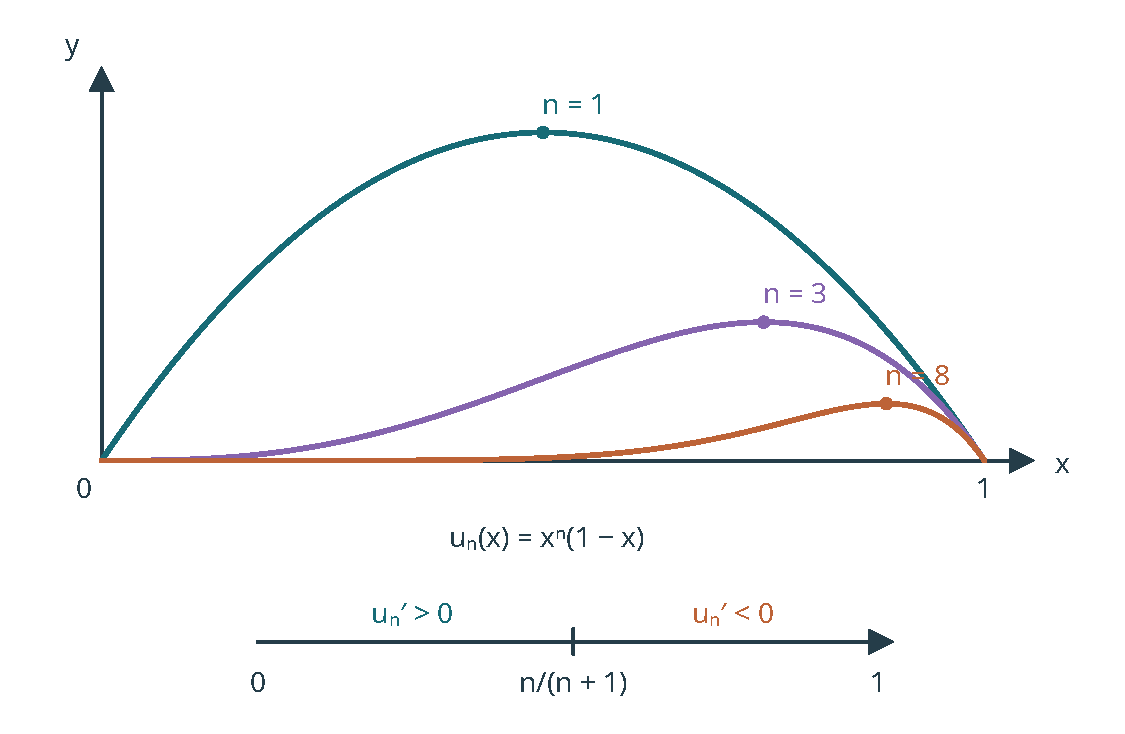
\includegraphics[width=0.85\linewidth]{figures/telescoping.pdf}
\captionof{figure}{Графики членов телескопического ряда и знак производной; максимум при x = n/(n + 1).}\label{fig-telescoping}
\end{minipage}
\end{center}

Однако частичные суммы телескопируются: \[
S_n(x)=\sum_{k=0}^n(x^k-x^{k+1})=1-x^{n+1}\longrightarrow
S(x)=\begin{cases}1,&0\le x<1,\\0,&x=1.\end{cases}
\] Сумма разрывна, хотя все частичные суммы непрерывны. Значит, равномерной сходимости нет. Более того, \(\lVert S_n-S\rVert_\infty=1\).

\end{example}

\section{Простейшие свойства и признаки}\label{sec-series-02}

\begin{theorem}[Линейность]\label{thm-series-linear}

Если \(\sum u_n\) и \(\sum v_n\) равномерно сходятся на \(\Omega\), то для \(\alpha,\beta\in\mathbb C\) \[
\sum_{n=1}^\infty(\alpha u_n+\beta v_n)
=\alpha\sum_{n=1}^\infty u_n+\beta\sum_{n=1}^\infty v_n,
\] причём ряд слева также сходится равномерно.

\end{theorem}

\begin{proof}

Применяем теорему \ref{thm-sequence-operations} к частичным суммам двух рядов.

\end{proof}

\begin{theorem}[Остатки ряда]\label{thm-series-tail}

Если \(\sum u_n\) сходится поточечно на \(\Omega\), то он сходится равномерно на \(\Omega\) тогда и только тогда, когда \(r_m\rightrightarrows0\) на \(\Omega\).

При каждом фиксированном \(m\) равномерная сходимость \(\sum_{n=1}^\infty u_n\) эквивалентна равномерной сходимости хвоста \(\sum_{n=m+1}^\infty u_n\).

\end{theorem}

\begin{proof}

Первое утверждение следует из формулы \eqref{eq-series-remainder}. Во втором при добавлении или удалении конечной суммы разность частичной суммы и предела не меняется.

\end{proof}

\begin{theorem}[Критерий Коши]\label{thm-series-cauchy}

Ряд \(\sum u_n(x)\) равномерно сходится на \(\Omega\) тогда и только тогда, когда

\begin{equation}
\forall\varepsilon>0\ \exists N\ \forall n>N\ \forall p\in\mathbb N:
\quad\sup_{x\in\Omega}\left|\sum_{k=n+1}^{n+p}u_k(x)\right|<\varepsilon.
\label{eq-series-cauchy}
\end{equation}

\end{theorem}

\begin{proof}

Необходимость следует из равномерной сходимости частичных сумм. Для достаточности условие даёт числовой критерий Коши в каждой точке, то есть предел \(S(x)\). Применяем оценку с \(\varepsilon/2\) и переходим к пределу \(p\to\infty\): \(\sup_x|S(x)-S_n(x)|\le\varepsilon/2<\varepsilon\).

Это рассуждение не требует ограниченности отдельных \(u_n\) или \(S_n\).

\end{proof}

\begin{theorem}[Признак Вейерштрасса]\label{thm-weierstrass}

Пусть \(|u_n(x)|\le a_n\) для всех \(x\in\Omega\), \(n\in\mathbb N\), где \(a_n\ge0\) и числовой ряд \(\sum a_n\) сходится. Тогда \(\sum u_n(x)\) сходится равномерно на \(\Omega\) и абсолютно в каждой точке \(\Omega\).

\end{theorem}

\begin{proof}

\[
\sup_{x\in\Omega}\left|\sum_{k=n+1}^{n+p}u_k(x)\right|
\le\sum_{k=n+1}^{n+p}a_k.
\] По критерию Коши для \(\sum a_n\) правая часть мала одновременно для всех \(p\). Применяем теорему \ref{thm-series-cauchy}. Для фиксированного \(x\) сходимость \(\sum|u_n(x)|\) следует из сравнения с \(\sum a_n\).

\end{proof}

Ряд \(\sum a_n\) называется \textbf{мажорирующим}. Естественный выбор \(a_n=\lVert u_n\rVert_\infty\) пригоден, если эти нормы конечны и их ряд сходится.

Мажоранты неотрицательны и вещественны: комплексная величина не может стоять справа в неравенстве \(|u_n(x)|\le a_n\).

\begin{example}[Мажоранта геометрического ряда]\label{exm-weierstrass-geometric}

На \([-q,q]\), \(0<q<1\), выполняется \(|x^n|\le q^n\). Ряд \(\sum_{n=1}^\infty q^n\) сходится, поэтому теорема \ref{thm-weierstrass} ещё раз даёт равномерную сходимость геометрического ряда.

На \((-1,1)\) тот же ряд сходится абсолютно в каждой точке, но не равномерно.

\end{example}

\begin{example}[Условная и равномерная сходимость]\label{exm-alternating-functional}

Ряд \[
\sum_{n=1}^\infty\frac{(-1)^{n+1}}{x^2+n},\qquad x\in\mathbb R,
\] сходится в каждой точке по признаку Лейбница. При этом \[
\lVert u_n\rVert_\infty=\frac1n\longrightarrow0,
\] но ряд из этих норм расходится, и признак Вейерштрасса неприменим.

Оценка остатка знакопеременного ряда даёт \[
|r_n(x)|\le\frac1{x^2+n+1}\le\frac1{n+1}.
\] Поэтому ряд всё же сходится равномерно на всей \(\mathbb R\).

Абсолютной сходимости нет ни в одной точке: при фиксированном \(x\) и достаточно больших \(n\) имеем \(x^2+n\le2n\), откуда \(1/(x^2+n)\ge1/(2n)\).

\end{example}

\begin{example}[Абсолютная сходимость не гарантирует равномерную]\label{exm-absolute-not-uniform}

Ряд \(\sum_{n=1}^\infty(1-x)x^n\) сходится абсолютно на \((-1,1]\): при \(|x|<1\) это геометрический ряд, при \(x=1\) все члены нулевые. Его сумма равна \(x\) при \(-1<x<1\) и нулю при \(x=1\). Она разрывна в \(1\), следовательно сходимость неравномерна.

\end{example}

Таким образом, абсолютная поточечная и равномерная сходимость не следуют друг из друга.

\begin{theorem}[Функциональная мажоранта]\label{thm-functional-majorant}

Если \(|u_n(x)|\le a_n(x)\), \(a_n(x)\ge0\), а \(\sum a_n(x)\) сходится равномерно на \(\Omega\), то \(\sum u_n(x)\) также сходится равномерно на \(\Omega\).

\end{theorem}

\begin{proof}

По формуле \eqref{eq-series-cauchy} и неотрицательности \(a_k\), \[
\sup_x\left|\sum_{k=n+1}^{n+p}u_k(x)\right|
\le\sup_x\sum_{k=n+1}^{n+p}a_k(x)\longrightarrow0
\] равномерно по \(p\).

\end{proof}

\section{Признаки Дирихле и Абеля}\label{sec-series-03}

В обоих признаках \(u_n\) могут быть комплекснозначными, а \(v_n\) --- \textbf{вещественными}, поскольку требуется монотонность по \(n\) в каждой точке \(x\).

\begin{theorem}[Признак Дирихле]\label{thm-dirichlet}

Пусть:

\begin{enumerate}
\def\labelenumi{\arabic{enumi}.}
\tightlist
\item
  Частичные суммы \(U_N(x)=\sum_{k=1}^N u_k(x)\) равномерно ограничены: \(|U_N(x)|\le C\) при всех \(N\) и \(x\in\Omega\).
\item
  Для каждого \(x\) последовательность \(v_n(x)\) монотонна по \(n\).
\item
  \(v_n\rightrightarrows0\) на \(\Omega\).
\end{enumerate}

Тогда \(\sum u_n(x)v_n(x)\) равномерно сходится на \(\Omega\).

\end{theorem}

\begin{proof}

Для хвоста от \(n+1\) до \(m\) обозначим \(A_k=\sum_{j=n+1}^k u_j\). Тогда \(|A_k|\le2C\). Преобразование Абеля: \[
\sum_{k=n+1}^m u_kv_k=A_mv_m+\sum_{k=n+1}^{m-1}A_k(v_k-v_{k+1}).
\] Монотонная последовательность, сходящаяся к нулю, имеет постоянный знак и убывающий модуль. Поэтому \[
\left|\sum_{k=n+1}^m u_k(x)v_k(x)\right|
\le2C\left(|v_m(x)|+\sum_{k=n+1}^{m-1}|v_k(x)-v_{k+1}(x)|\right)
=2C|v_{n+1}(x)|.
\] Правая часть стремится к нулю равномерно по \(x\), независимо от \(m>n\). Применяем теорему \ref{thm-series-cauchy}.

\end{proof}

\begin{theorem}[Признак Абеля]\label{thm-abel-test}

Пусть \(\sum u_n(x)\) равномерно сходится на \(\Omega\), \(v_n(x)\) монотонна по \(n\) для каждого \(x\), а \(|v_n(x)|\le C\) для всех \(n\) и \(x\). Тогда \(\sum u_n(x)v_n(x)\) равномерно сходится на \(\Omega\).

\end{theorem}

\begin{proof}

По критерию Коши при достаточно большом \(n\) все хвостовые суммы \(A_k=\sum_{j=n+1}^k u_j\) удовлетворяют \(|A_k(x)|<\eta\) одновременно для всех \(k>n\) и \(x\). То же преобразование Абеля и монотонность дают \[
\left|\sum_{k=n+1}^m u_kv_k\right|
\le\eta\left(|v_m|+|v_{n+1}-v_m|\right)\le3C\eta.
\] Выбираем \(\eta=\varepsilon/(3C)\) при \(C>0\); случай \(C=0\) тривиален.

\end{proof}

\section{Функциональные свойства суммы ряда}\label{sec-series-04}

\begin{theorem}[Непрерывность суммы]\label{thm-series-continuity}

Если все \(u_n\in C(\Omega)\), а \(\sum u_n\) сходится равномерно на \(\Omega\), то \(S=\sum u_n\in C(\Omega)\).

\end{theorem}

\begin{proof}

Частичные суммы непрерывны и сходятся равномерно. Применяем теорему \ref{thm-continuity-sequence}.

\end{proof}

\begin{cor}[Предельный переход под знаком ряда]\label{cor-series-limit}

Пусть \(\sum u_n\) сходится равномерно на \(\Omega\), \(x_0\) --- предельная точка \(\Omega\), а для каждого \(n\) существует конечный \(a_n=\lim_{x\to x_0}u_n(x)\). Тогда \(\sum a_n\) сходится и \[
\lim_{x\to x_0}\sum_{n=1}^\infty u_n(x)
=\sum_{n=1}^\infty\lim_{x\to x_0}u_n(x)=\sum_{n=1}^\infty a_n.
\]

\end{cor}

\begin{proof}

Для частичных сумм \(S_n\) имеем \(\lim_{x\to x_0}S_n(x)=\sum_{k=1}^n a_k=A_n\). Применяем следствие \ref{cor-interchange-limits} к \(S_n\rightrightarrows S\).

\end{proof}

\begin{theorem}[Почленное интегрирование]\label{thm-series-integral}

Пусть \(u_n:[a,b]\to\mathbb R\), \(a<b\), все \(u_n\in R([a,b])\), а \(\sum u_n\) сходится равномерно на \([a,b]\). Тогда \(S\in R([a,b])\) и

\begin{equation}
\int_a^b S(x)\,dx=\sum_{n=1}^\infty\int_a^b u_n(x)\,dx.
\label{eq-series-integral}
\end{equation}

\end{theorem}

\begin{proof}

Применяем теорему \ref{thm-integrate-sequence} к частичным суммам и используем линейность интеграла для конечных сумм.

\end{proof}

\begin{theorem}[Почленное дифференцирование]\label{thm-series-derivative}

Пусть \(u_n:[a,b]\to\mathbb R\) дифференцируемы, ряд \(\sum u_n'\) сходится равномерно на \([a,b]\), а \(\sum u_n(x_0)\) сходится хотя бы в одной точке \(x_0\in[a,b]\). Тогда \(\sum u_n\) сходится равномерно на \([a,b]\), его сумма дифференцируема и

\begin{equation}
S'(x)=\left(\sum_{n=1}^\infty u_n(x)\right)'
=\sum_{n=1}^\infty u_n'(x).
\label{eq-series-derivative}
\end{equation}

На концах отрезка производные односторонние.

\end{theorem}

\begin{proof}

Применяем теорему \ref{thm-differentiate-sequence} к \(S_n=\sum_{k=1}^n u_k\): \(S_n'=\sum_{k=1}^n u_k'\) сходится равномерно, а \(S_n(x_0)\) имеет конечный предел.

\end{proof}


\part{Степенные ряды}\label{sec-power-series}
\section{Общие понятия. Первая теорема Абеля}\label{sec-power-series-01}

\begin{definition}[Степенной ряд]\label{def-power-series}

Ряд вида

\begin{equation}
\sum_{n=0}^\infty c_n(z-z_0)^n,
\qquad c_n,z_0\in\mathbb C,
\label{eq-power-series}
\end{equation}

называется степенным рядом с центром \(z_0\). В вещественном случае \(c_n,z_0,z\in\mathbb R\).

Сдвиг \(w=z-z_0\) сводит его к ряду \(\sum_{n=0}^\infty c_nw^n\) с центром в нуле.

\end{definition}

\begin{theorem}[Первая теорема Абеля]\label{thm-abel-first}

Для ряда \(\sum c_nz^n\):

\begin{enumerate}
\def\labelenumi{\arabic{enumi}.}
\tightlist
\item
  Если ряд сходится в точке \(a\ne0\), то он сходится абсолютно при \(|z|<|a|\) и равномерно на каждом замкнутом круге \(|z|\le r<|a|\).
\item
  Если ряд расходится в точке \(b\), то он расходится при всех \(|z|>|b|\).
\end{enumerate}

\end{theorem}

Весь открытый круг \(|z|<|a|\) не обязан быть множеством равномерной сходимости.

\begin{proof}

\textbf{1.} Из сходимости \(\sum c_na^n\) следует \(c_na^n\to0\), поэтому существует \(M>0\) с \(|c_na^n|\le M\) для всех \(n\). При \(|z|\le r<|a|\) положим \(q=r/|a|<1\). Тогда \[
|c_nz^n|=|c_na^n|\left|\frac za\right|^n\le Mq^n.
\] Ряд \(\sum Mq^n\) сходится. По теореме \ref{thm-weierstrass} получаем равномерную сходимость на \(|z|\le r\) и абсолютную в каждой его точке. Любая точка \(|z|<|a|\) попадает в такой круг.

\textbf{2.} Если бы ряд сходился в точке \(z_1\) с \(|z_1|>|b|\), то по первой части он сходился бы в \(b\). Противоречие.

\end{proof}

\begin{definition}[Радиус сходимости]\label{def-radius}

Радиус сходимости ряда \eqref{eq-power-series} определяется как \[
R=\sup\left\{|w|:\ \sum_{n=0}^\infty c_nw^n\text{ сходится}\right\},
\qquad 0\le R\le+\infty.
\] При \(|z-z_0|<R\) ряд сходится абсолютно, при \(|z-z_0|>R\) расходится. На границе \(|z-z_0|=R\) требуется отдельное исследование.

В вещественном случае \((x_0-R,x_0+R)\) называется интервалом сходимости; его концы не включаются в это название независимо от сходимости в них.

\end{definition}

\begin{center}
\begin{minipage}{\linewidth}
\centering
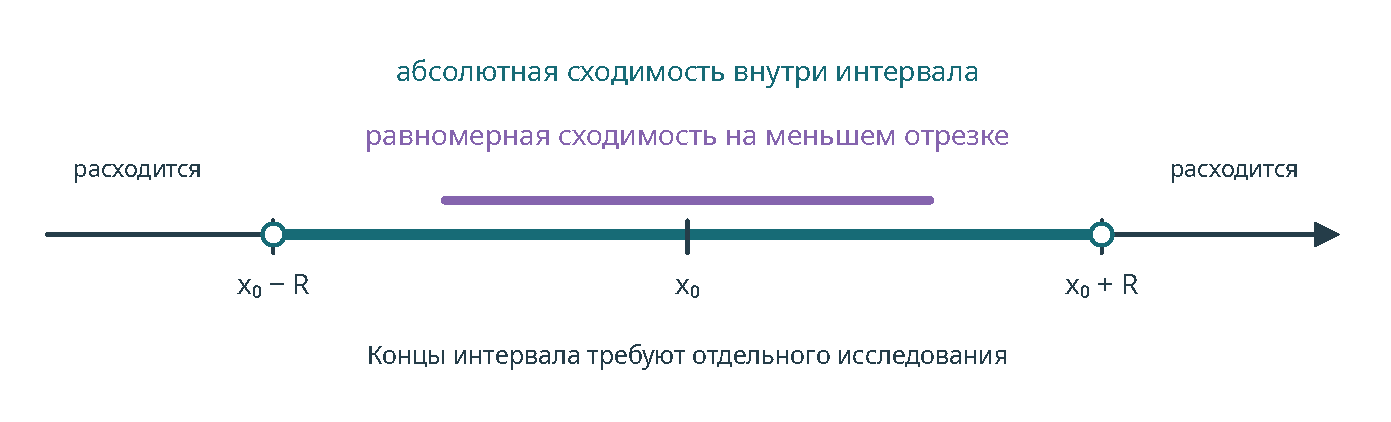
\includegraphics[width=0.95\linewidth]{figures/interval.pdf}
\captionof{figure}{Интервал сходимости и меньший отрезок равномерной сходимости.}\label{fig-interval}
\end{minipage}
\end{center}

\section{Формулы для радиуса сходимости}\label{sec-power-series-02}

\begin{theorem}[Формула Коши--Адамара]\label{thm-cauchy-hadamard}

Для ряда \eqref{eq-power-series}

\begin{equation}
\frac1R=\limsup_{n\to\infty}\sqrt[n]{|c_n|}.
\label{eq-cauchy-hadamard}
\end{equation}

Принимаются соглашения \(1/0=+\infty\) и \(1/(+\infty)=0\).

\end{theorem}

\begin{proof}

Сдвигом полагаем \(z_0=0\) и обозначаем \(L=\limsup_n\sqrt[n]{|c_n|}\).

\textbf{Случай \(L=0\).} Для каждого фиксированного \(z\) имеем \[
\sqrt[n]{|c_nz^n|}=|z|\sqrt[n]{|c_n|}\longrightarrow0.
\] По коренному признаку Коши ряд сходится абсолютно при всех \(z\), то есть \(R=+\infty\).

\textbf{Случай \(L=+\infty\).} Для каждого \(z\ne0\) существует подпоследовательность \(n_k\), для которой \(|z|\sqrt[n_k]{|c_{n_k}|}\to+\infty\). Тогда члены \(c_{n_k}z^{n_k}\) не стремятся к нулю. Ряд расходится при \(z\ne0\), а при \(z=0\) равен \(c_0\). Значит, \(R=0\).

\textbf{Случай \(0<L<+\infty\).} Если \(|z|<1/L\), выбираем \(\eta>0\) так, чтобы \(|z|(L+\eta)<1\). По определению верхнего предела для всех достаточно больших \(n\), \[
\sqrt[n]{|c_n|}<L+\eta,
\qquad\sqrt[n]{|c_nz^n|}<|z|(L+\eta)<1.
\] По признаку Коши ряд сходится абсолютно.

Если \(|z|>1/L\), выбираем \(0<\eta<L\) с \(|z|(L-\eta)>1\). По определению верхнего предела существует бесконечная подпоследовательность \(n_k\) с \(\sqrt[n_k]{|c_{n_k}|}>L-\eta\). Вдоль неё \[
\sqrt[n_k]{|c_{n_k}z^{n_k}|}>|z|(L-\eta)>1,
\] так что необходимое условие сходимости нарушено. Следовательно, \(R=1/L\).

\end{proof}

\begin{cor}[Частные формулы]\label{cor-radius-limits}

Если существует предел \(\lim_n\sqrt[n]{|c_n|}\), то его можно использовать вместо верхнего предела в формуле \eqref{eq-cauchy-hadamard}.

Если коэффициенты \(c_n\) ненулевые начиная с некоторого номера и существует (в том числе бесконечный) предел отношений, то

\begin{equation}
\frac1R=\lim_{n\to\infty}\frac{|c_{n+1}|}{|c_n|}.
\label{eq-radius-ratio}
\end{equation}

\end{cor}

Условие о ненулевых коэффициентах нужно, чтобы отношения были определены. Ряды с пропущенными степенями следует проверять непосредственно или по формуле \eqref{eq-cauchy-hadamard}.

\section{Свойства степенных рядов}\label{sec-power-series-03}

\begin{theorem}[Сходимость внутри круга]\label{thm-power-uniform}

Пусть \(R>0\) --- радиус ряда \eqref{eq-power-series}. Для каждого \(0<r<R\) ряд сходится равномерно на \(|z-z_0|\le r\) и абсолютно в каждой точке \(|z-z_0|<R\).

\end{theorem}

\begin{proof}

По определению \(R\) существует точка сходимости, расстояние которой от центра больше \(r\). Применяем теорему \ref{thm-abel-first}.

\end{proof}

\begin{theorem}[Непрерывность суммы]\label{thm-power-continuity}

Сумма \(S(z)=\sum_{n=0}^\infty c_n(z-z_0)^n\) непрерывна внутри круга \(|z-z_0|<R\).

\end{theorem}

\begin{proof}

Для любой точки \(z^*\) внутри круга выбираем \(r\) с \(|z^*-z_0|<r<R\). На \(|z-z_0|\le r\) ряд сходится равномерно, а каждый его член непрерывен. По теореме \ref{thm-series-continuity} сумма непрерывна в \(z^*\).

\end{proof}

\begin{center}
\begin{minipage}{\linewidth}
\centering
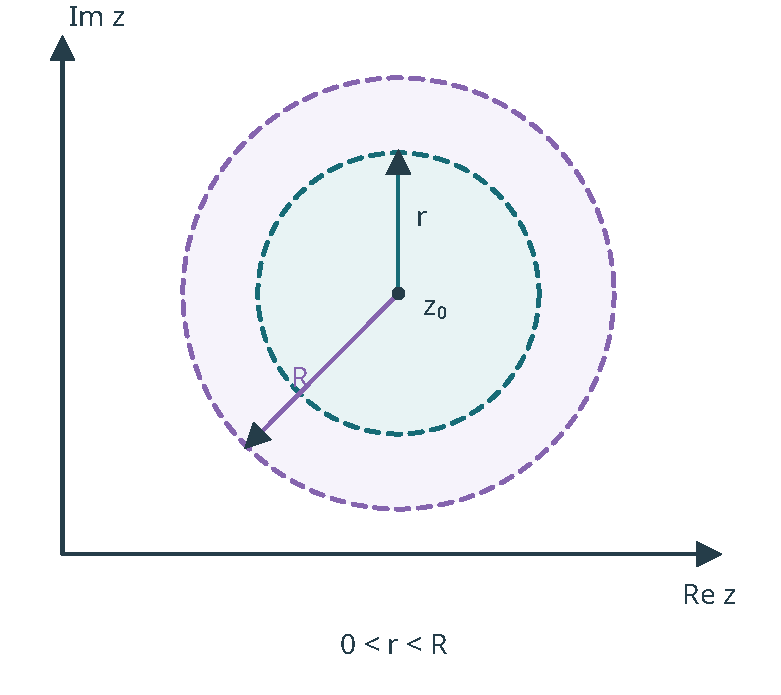
\includegraphics[width=0.65\linewidth]{figures/disks.pdf}
\captionof{figure}{Круг сходимости радиуса R и вложенный круг радиуса r с равномерной сходимостью.}\label{fig-disks}
\end{minipage}
\end{center}

\begin{cor}[Вторая теорема Абеля: радиальный предел]\label{cor-abel-second}

Пусть \(0<R<+\infty\) и ряд сходится в граничной точке \(z^*\), \(|z^*-z_0|=R\). Тогда

\begin{equation}
\lim_{t\to1-}S\bigl(z_0+t(z^*-z_0)\bigr)=S(z^*),
\qquad 0\le t<1.
\label{eq-abel-radial}
\end{equation}

В вещественном случае это непрерывность суммы при подходе к концу интервала изнутри.

\end{cor}

При условной сходимости на границе гарантируется радиальный предел. Если \(\sum|c_n|R^n<\infty\), то по Вейерштрассу ряд равномерно сходится на замкнутом круге и сумма непрерывна на всей его границе.

\begin{proof}

Обозначим \(b_n=c_n(z^*-z_0)^n\). Числовой ряд \(\sum b_n\) сходится. Рассматриваем его как функциональный ряд постоянных функций на \([0,1]\): он сходится равномерно. Множители \(v_n(t)=t^n\) монотонны по \(n\) при каждом \(t\in[0,1]\) и ограничены единицей. По теореме \ref{thm-abel-test} ряд \(\sum b_nt^n\) сходится равномерно на \([0,1]\). Его сумма непрерывна, что даёт формулу \eqref{eq-abel-radial}.

\end{proof}

\subsection{Дифференцирование}\label{sec-power-series-03-1}

\begin{theorem}[Производная суммы степенного ряда]\label{thm-power-derivative}

Внутри круга сходимости

\begin{equation}
S'(z)=\sum_{n=1}^\infty nc_n(z-z_0)^{n-1}.
\label{eq-power-derivative}
\end{equation}

Радиус производного ряда равен \(R\), а \(S'\) непрерывна внутри круга.

\end{theorem}

\begin{proof}

Сдвигом полагаем \(z_0=0\). Сначала ряд \(\sum_{n=1}^\infty nc_nz^n\) имеет тот же радиус, поскольку \(n^{1/n}\to1\): \[
\limsup_n\sqrt[n]{n|c_n|}=\limsup_n\sqrt[n]{|c_n|}=1/R.
\] Сдвиг показателя степени на единицу также сохраняет радиус: при \(z\ne0\) ряд \(\sum nc_nz^{n-1}\) --- это \(z^{-1}\sum nc_nz^n\); в нуле оба ряда определены. Поэтому производный ряд имеет радиус \(R\).

Фиксируем \(z^*\) с \(|z^*|<R\) и выбираем \(r\) с \(|z^*|<r<R\). Для \(z\ne z^*\), \[
\frac{S(z)-S(z^*)}{z-z^*}
=\sum_{n=1}^\infty c_n\frac{z^n-(z^*)^n}{z-z^*}.
\] Каждый член справа продолжается в \(z=z^*\) как полином \[
u_n(z)=c_n\bigl(z^{n-1}+z^{n-2}z^*+\cdots+(z^*)^{n-1}\bigr).
\] При \(|z|\le r\), \(|z^*|<r\) получаем \(|u_n(z)|\le|c_n|nr^{n-1}\). Числовой ряд этих мажорант сходится, поскольку \(r<R\). По теореме \ref{thm-weierstrass} ряд \(\sum u_n(z)\) сходится равномерно и имеет непрерывную сумму. Поэтому \[
\lim_{z\to z^*}\frac{S(z)-S(z^*)}{z-z^*}
=\sum_{n=1}^\infty\lim_{z\to z^*}u_n(z)
=\sum_{n=1}^\infty nc_n(z^*)^{n-1}.
\] Непрерывность \(S'\) следует из теоремы \ref{thm-power-continuity} для производного ряда.

\end{proof}

\begin{cor}[Производные всех порядков]\label{cor-power-higher-derivatives}

Сумма степенного ряда бесконечно дифференцируема внутри круга сходимости, и для каждого \(k\ge0\)

\begin{equation}
S^{(k)}(z)=\sum_{n=k}^\infty c_n\frac{n!}{(n-k)!}(z-z_0)^{n-k}.
\label{eq-power-higher-derivatives}
\end{equation}

Все эти производные непрерывны внутри круга.

\end{cor}

Доказательство --- последовательное применение теоремы \ref{thm-power-derivative}.

\subsection{Интегрирование}\label{sec-power-series-03-2}

\begin{theorem}[Почленное интегрирование вещественного ряда]\label{thm-power-integral}

Пусть \(S(x)=\sum_{n=0}^\infty c_n(x-x_0)^n\), где \(c_n,x_0\in\mathbb R\), \(R>0\). Если \([a,b]\subset(x_0-R,x_0+R)\), то \(S\in R([a,b])\) и

\begin{equation}
\begin{aligned}
\int_a^b S(x)\,dx
&=\sum_{n=0}^\infty c_n\int_a^b \bigl((x-x_0)^n\bigr)\,dx\\
&=\sum_{n=0}^\infty\frac{c_n}{n+1}
\left((b-x_0)^{n+1}-(a-x_0)^{n+1}\right).
\end{aligned}
\label{eq-power-integral}
\end{equation}

\end{theorem}

\begin{proof}

Отрезок \([a,b]\) содержится в меньшем отрезке \(|x-x_0|\le r<R\). Ряд на нём сходится равномерно. Применяем теорему \ref{thm-series-integral}.

\end{proof}

\section{Разложение функции. Ряд Тейлора}\label{sec-power-series-04}

\begin{theorem}[Коэффициенты разложения]\label{thm-power-coefficients}

Если \(S(z)=\sum_{n=0}^\infty c_n(z-z_0)^n\) имеет положительный радиус сходимости, то

\begin{equation}
c_n=\frac{S^{(n)}(z_0)}{n!},\qquad n\ge0.
\label{eq-taylor-coefficients}
\end{equation}

\end{theorem}

\begin{proof}

\(S(z_0)=c_0\). В формуле \eqref{eq-power-higher-derivatives} подставляем \(z=z_0\): единственный ненулевой член соответствует \(n=k\), поэтому \(S^{(k)}(z_0)=k!c_k\).

\end{proof}

\begin{cor}[Единственность разложения]\label{cor-power-uniqueness}

Если на некотором круге \(|z-z_0|<r\), \(r>0\), \[
\sum_{n=0}^\infty a_n(z-z_0)^n
=\sum_{n=0}^\infty b_n(z-z_0)^n,
\] то \(a_n=b_n\) для всех \(n\ge0\).

\end{cor}

Это следует из формулы \eqref{eq-taylor-coefficients}. Для ряда с центром в нуле: если сумма чётна, все коэффициенты нечётных степеней равны нулю; если нечётна, все коэффициенты чётных степеней равны нулю.

При другом центре нужно рассматривать симметрию относительно \(z_0\).

\begin{definition}[Ряд Тейлора и ряд Маклорена]\label{def-taylor-series}

Функции \(f\), имеющей производные всех порядков в точке \(z_0\), сопоставляют ряд

\begin{equation}
\sum_{n=0}^\infty\frac{f^{(n)}(z_0)}{n!}(z-z_0)^n.
\label{eq-taylor-series}
\end{equation}

Он называется рядом Тейлора функции в точке \(z_0\), а при \(z_0=0\) --- рядом Маклорена.

\end{definition}

Для вещественной бесконечно дифференцируемой функции радиус этого ряда и совпадение его суммы с \(f\) требуют отдельного исследования. Любой сходящийся степенной ряд является рядом Тейлора своей суммы.

Для комплексной функции, голоморфной в окрестности, разложение в ряд Тейлора там существует. Предостережение о несовпадении суммы с функцией относится к общему вещественному \(C^\infty\)-случаю.

\begin{definition}[Аналитичность]\label{def-analytic}

Функция называется аналитической (регулярной) в точке \(z_0\), если в некоторой её окрестности допускает представление сходящимся степенным рядом с центром \(z_0\).

\end{definition}

\subsection{Достаточные условия разложения вещественной функции}\label{sec-power-series-04-1}

\begin{theorem}[Оценки производных]\label{thm-taylor-sufficient}

Пусть \(f:\mathbb R\to\mathbb R\) бесконечно дифференцируема в окрестности отрезка \(|x-x_0|\le r\), \(r>0\). Каждого из следующих условий достаточно для совпадения \(f\) со своим рядом Тейлора на этом отрезке:

\begin{enumerate}
\def\labelenumi{\arabic{enumi}.}
\tightlist
\item
  \(0<r<1\) и существует \textbf{одна} константа \(M>0\) такая, что \(|f^{(n)}(x)|\le M n!\) для всех \(n\ge0\) и всех \(|x-x_0|\le r\).
\item
  Существует \textbf{одна} константа \(M>0\) такая, что \(|f^{(n)}(x)|\le M\) для всех \(n\ge0\) и всех \(|x-x_0|\le r\).
\end{enumerate}

\end{theorem}

\begin{proof}

По формуле Тейлора с остатком Лагранжа при некотором \(c\) между \(x\) и \(x_0\), \[
f(x)-\sum_{k=0}^{n-1}\frac{f^{(k)}(x_0)}{k!}(x-x_0)^k
=\frac{f^{(n)}(c)}{n!}(x-x_0)^n.
\] В первом случае модуль остатка не превосходит \(Mr^n\to0\), во втором --- \(Mr^n/n!\to0\). Оценки равномерны по \(|x-x_0|\le r\). Поэтому в обоих случаях \[
f(x)=\sum_{k=0}^\infty\frac{f^{(k)}(x_0)}{k!}(x-x_0)^k.
\]

\end{proof}

\section{Ряды Маклорена основных функций}\label{sec-power-series-05}

\subsection{Экспонента}\label{sec-power-series-05-1}

\begin{equation}
e^z=\sum_{n=0}^\infty\frac{z^n}{n!},\qquad R=+\infty.
\label{eq-exp-series}
\end{equation}

По формуле отношений: \(|c_{n+1}|/|c_n|=1/(n+1)\to0\).

\subsection{Синус и косинус}\label{sec-power-series-05-2}

\begin{equation}
\sin z=\sum_{n=0}^\infty\frac{(-1)^n}{(2n+1)!}z^{2n+1},\qquad R=+\infty,
\label{eq-sin-series}
\end{equation}

\begin{equation}
\cos z=\sum_{n=0}^\infty\frac{(-1)^n}{(2n)!}z^{2n},\qquad R=+\infty.
\label{eq-cos-series}
\end{equation}

Для фиксированного \(z\) отношение модулей соседних ненулевых членов стремится к нулю. Нулевые коэффициенты пропущенных степеней не позволяют напрямую применять формулу \eqref{eq-radius-ratio} ко всем коэффициентам.

\subsection{Логарифм}\label{sec-power-series-05-3}

\begin{equation}
\log(1+z)=\sum_{n=1}^\infty\frac{(-1)^{n+1}z^n}{n},\qquad R=1.
\label{eq-log-series}
\end{equation}

В комплексном круге \(|z|<1\) выбирается ветвь логарифма с \(\log1=0\). В вещественном случае это \(\ln(1+x)\).

Радиус равен единице, поскольку \(\sqrt[n]{1/n}\to1\). В концах вещественного интервала:

\begin{itemize}
\tightlist
\item
  При \(x=-1\) получаем \(-\sum 1/n\), то есть расходимость.
\item
  При \(x=1\) получаем \(\sum(-1)^{n+1}/n\), то есть условную сходимость по Лейбницу; по следствию \ref{cor-abel-second} сумма равна \(\ln2\).
\end{itemize}

\begin{center}
\begin{minipage}{\linewidth}
\centering
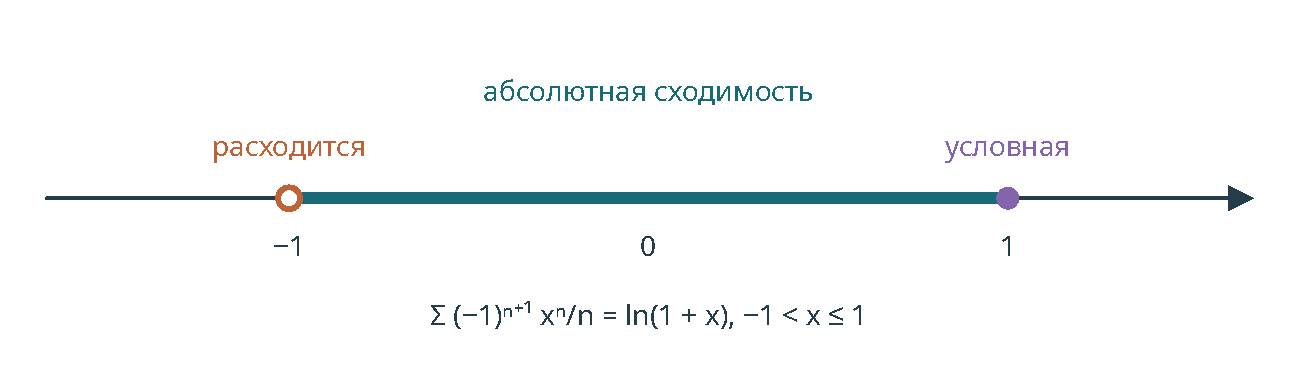
\includegraphics[width=0.95\linewidth]{figures/log-interval.pdf}
\captionof{figure}{Для ряда логарифма: расходимость при −1, абсолютная сходимость внутри и условная при 1.}\label{fig-log-interval}
\end{minipage}
\end{center}

\subsection{Биномиальный ряд}\label{sec-power-series-05-4}

\begin{equation}
(1+x)^p=\sum_{n=0}^\infty\binom pn x^n,
\qquad\binom p0=1,\quad
\binom pn=\frac{p(p-1)\cdots(p-n+1)}{n!}\ (n\ge1).
\label{eq-binomial-series}
\end{equation}

Для \(p\in\mathbb R\setminus\{0,1,2,\ldots\}\) радиус равен \(1\), поскольку \[
\left|\frac{c_{n+1}}{c_n}\right|=\left|\frac{p-n}{n+1}\right|\longrightarrow1.
\] Равенство выполняется при \(|x|<1\); сходимость в концах требует отдельного исследования.

Если \(p\) --- неотрицательное целое число, ряд обрывается и является многочленом; тогда \(R=+\infty\). Для \(n=0\) произведение в числителе пустое и равно единице.

На вещественных отрезках разложения экспоненты, синуса и косинуса следуют из формулы Тейлора и оценки остатка; комплексные формулы задают их стандартные целые продолжения. Для логарифма можно проинтегрировать геометрический ряд \(1/(1+x)=\sum_{n\ge0}(-x)^n\) на отрезке внутри \((-1,1)\). Для биномиального ряда коэффициенты удовлетворяют \((n+1)c_{n+1}=(p-n)c_n\). Поэтому его сумма \(B\) решает \((1+x)B'=pB\), \(B(0)=1\); на \((-1,1)\) отсюда \(B=(1+x)^p\).


\part{Ряды Фурье}\label{sec-fourier}
\section{Ортогональные системы функций}\label{sec-fourier-orthogonal}

Здесь рассматриваются вещественные функции на отрезке \([a,b]\), \(a<b\). Интегралы понимаются по Риману; далее также допускаются абсолютно сходящиеся несобственные интегралы с конечным числом особых точек.

\begin{definition}[Скалярное произведение и норма]\label{def-function-inner-product}

Для \(f,g\in C([a,b])\) положим
\begin{equation}
(f,g)=\int_a^b f(x)g(x)\,dx,
\qquad
\|f\|=\sqrt{(f,f)}=\left(\int_a^b f^2(x)\,dx\right)^{1/2}.
\label{eq-function-inner-product}
\end{equation}
Это скалярное произведение и порождённая им норма на \(C([a,b])\).

\end{definition}

Действительно, симметрия и билинейность следуют из свойств интеграла. Если непрерывная функция \(f\) ненулевая хотя бы в одной точке, то \(f^2\) положительна на некотором участке отрезка, поэтому \((f,f)>0\).

\begin{definition}[Ортогональная система]\label{def-orthogonal-system}

Система ненулевых функций \(\varphi_1,\varphi_2,\ldots\in C([a,b])\) называется ортогональной на \([a,b]\), если
\[
(\varphi_n,\varphi_m)=\int_a^b\varphi_n(x)\varphi_m(x)\,dx=0
\qquad(n\ne m).
\]
Для каждого \(n\) имеем \(\|\varphi_n\|^2>0\).

\end{definition}

\begin{example}[Тригонометрическая система]\label{exm-trigonometric-system}

Система
\[
1,\ \sin x,\ \cos x,\ \sin 2x,\ \cos 2x,\ldots
\]
ортогональна на \([-\pi,\pi]\). Для \(n,m\ge1\) справедливы равенства
\begin{equation}
\begin{aligned}
\int_{-\pi}^{\pi}\sin nx\cos mx\,dx&=0,\\
\int_{-\pi}^{\pi}\cos nx\cos mx\,dx
&=\begin{cases}0,&n\ne m,\\ \pi,&n=m,\end{cases}\\
\int_{-\pi}^{\pi}\sin nx\sin mx\,dx
&=\begin{cases}0,&n\ne m,\\ \pi,&n=m.\end{cases}
\end{aligned}
\label{eq-trigonometric-orthogonality}
\end{equation}
Кроме того,
\[
\int_{-\pi}^{\pi}\cos nx\,dx
=\int_{-\pi}^{\pi}\sin nx\,dx=0,
\qquad
\|1\|^2=2\pi,\quad
\|\cos nx\|^2=\|\sin nx\|^2=\pi.
\]

\end{example}

\begin{proof}

Произведение \(\sin nx\cos mx\) нечётно, поэтому его интеграл на симметричном отрезке равен нулю. Используем формулы
\[
\begin{aligned}
\cos nx\cos mx&=\tfrac12\bigl(\cos(n-m)x+\cos(n+m)x\bigr),\\
\sin nx\sin mx&=\tfrac12\bigl(\cos(n-m)x-\cos(n+m)x\bigr).
\end{aligned}
\]
Интеграл \(\cos kx\) на \([-\pi,\pi]\) равен нулю при целом \(k\ne0\) и равен \(2\pi\) при \(k=0\). Это даёт все равенства \eqref{eq-trigonometric-orthogonality} и значения норм. Ортогональность постоянной функции остальным следует из интегралов синуса и косинуса.\qedhere

\end{proof}

\begin{example}[Многочлены Лежандра]\label{exm-legendre-system}

Другой пример ортогональной системы на \([-1,1]\) --- многочлены Лежандра:
\begin{equation}
L_n(x)=\frac1{2^n n!}\frac{d^n}{dx^n}(x^2-1)^n,
\qquad n=0,1,2,\ldots
\label{eq-legendre-rodrigues}
\end{equation}
Это формула Родрига. Например, \(L_0(x)=1\), \(L_1(x)=x\), \(L_2(x)=(3x^2-1)/2\).

\end{example}

\section{Коэффициенты и ряды Фурье}\label{sec-fourier-coefficients}

\begin{lemma}[Коэффициенты равномерного разложения]\label{lem-orthogonal-coefficients}

Пусть \(\{\varphi_n\}\) --- ортогональная система на \([a,b]\), а ряд \(\sum_{n=1}^\infty c_n\varphi_n(x)\) сходится равномерно на этом отрезке к \(f(x)\). Тогда
\begin{equation}
c_n=\frac{(f,\varphi_n)}{\|\varphi_n\|^2}
=\frac{\displaystyle\int_a^b f(x)\varphi_n(x)\,dx}
{\displaystyle\int_a^b\varphi_n^2(x)\,dx},
\qquad n\ge1.
\label{eq-orthogonal-coefficients}
\end{equation}

\end{lemma}

\begin{proof}

Фиксируем \(k\). Непрерывная функция \(\varphi_k\) ограничена на \([a,b]\). Умножение равномерно сходящегося ряда на неё сохраняет равномерную сходимость. По теореме \ref{thm-series-integral} можно интегрировать почленно:
\[
\begin{aligned}
(f,\varphi_k)
&=\int_a^b\left(\sum_{n=1}^\infty c_n\varphi_n(x)\right)\varphi_k(x)\,dx\\
&=\sum_{n=1}^\infty c_n\int_a^b\varphi_n(x)\varphi_k(x)\,dx
=c_k\|\varphi_k\|^2.
\end{aligned}
\]
При \(n\ne k\) интегралы равны нулю по ортогональности. Делим на положительное число \(\|\varphi_k\|^2\).

\end{proof}

\begin{definition}[Ряд Фурье по ортогональной системе]\label{def-orthogonal-fourier-series}

Пусть \(f\in C([a,b])\). Числа \(c_n\), определённые формулой \eqref{eq-orthogonal-coefficients}, называются коэффициентами Фурье функции \(f\) по системе \(\{\varphi_n\}\). Ряд \(\sum_{n=1}^\infty c_n\varphi_n(x)\) называется её рядом Фурье по этой системе. Записывают
\[
f(x)\sim\sum_{n=1}^\infty c_n\varphi_n(x).
\]
Знак \(\sim\) означает соответствие функции её ряду Фурье; сходимость ряда и равенство его суммы функции требуют отдельного исследования.

\end{definition}

Формула коэффициентов применима и к интегрируемым по Риману функциям \(f\): непрерывность \(\varphi_n\) обеспечивает существование интегралов. Также можно допустить абсолютно сходящиеся несобственные интегралы, если \(f\) локально интегрируема внутри \((a,b)\).

\subsection{Тригонометрический ряд Фурье}\label{sec-fourier-trigonometric}

\begin{definition}[Тригонометрические коэффициенты]\label{def-trigonometric-fourier-series}

Пусть \(f\) абсолютно интегрируема на \([-\pi,\pi]\) в собственном или несобственном смысле. Её тригонометрический ряд Фурье имеет вид
\begin{equation}
f(x)\sim\frac{a_0}{2}+\sum_{n=1}^\infty\bigl(a_n\cos nx+b_n\sin nx\bigr),
\label{eq-trigonometric-fourier-series}
\end{equation}
где
\begin{equation}
\begin{aligned}
a_n&=\frac1\pi\int_{-\pi}^{\pi}f(x)\cos nx\,dx,\qquad n\ge0,\\
b_n&=\frac1\pi\int_{-\pi}^{\pi}f(x)\sin nx\,dx,\qquad n\ge1.
\end{aligned}
\label{eq-trigonometric-coefficients}
\end{equation}

\end{definition}

Значения норм в примере \ref{exm-trigonometric-system} объясняют множитель \(1/\pi\). Коэффициент при постоянной функции равен \((f,1)/\|1\|^2=(2\pi)^{-1}\int_{-\pi}^{\pi}f(x)\,dx=a_0/2\), откуда отдельная запись постоянного члена.

\section{Лемма Римана об осциллирующих интегралах}\label{sec-fourier-riemann}

Обозначение \(f\in R_{\mathrm{loc}}((a,b))\) означает, что \(f\) интегрируема по Риману на каждом замкнутом отрезке, лежащем внутри \((a,b)\). Абсолютная интегрируемость означает конечность \(\int_a^b|f(x)|\,dx\); при особых точках этот интеграл понимается как несобственный.

\begin{lemma}[Римана]\label{lem-riemann-oscillatory}

Пусть \((a,b)\) --- конечный или бесконечный интервал, \(f\in R_{\mathrm{loc}}((a,b))\), а \(\int_a^b|f(x)|\,dx<+\infty\). Тогда
\begin{equation}
\lim_{|\omega|\to\infty}\int_a^b f(x)\sin\omega x\,dx
=\lim_{|\omega|\to\infty}\int_a^b f(x)\cos\omega x\,dx=0.
\label{eq-riemann-oscillatory}
\end{equation}

\end{lemma}

\begin{proof}

\textbf{1. Собственный интеграл на конечном отрезке.}
Пусть \(f\in R([a,b])\) и \(|f(x)|\le C\). Для \(\varepsilon>0\) выбираем разбиение \(a=x_0<x_1<\cdots<x_N=b\), для которого разность верхней и нижней сумм Дарбу удовлетворяет
\[
\sum_{j=1}^N(M_j-m_j)\Delta x_j<\frac{\varepsilon}{2},
\]
где \(M_j=\sup_{[x_{j-1},x_j]}f\), \(m_j=\inf_{[x_{j-1},x_j]}f\), \(\Delta x_j=x_j-x_{j-1}\).
На каждом участке вычитаем постоянную \(m_j\). При \(\omega\ne0\) получаем
\[
\begin{aligned}
\left|\int_a^b f(x)\sin\omega x\,dx\right|
&\le\sum_{j=1}^N\int_{x_{j-1}}^{x_j}|f(x)-m_j|\,dx
+\sum_{j=1}^N|m_j|\left|\int_{x_{j-1}}^{x_j}\sin\omega x\,dx\right|\\
&\le\sum_{j=1}^N(M_j-m_j)\Delta x_j
+\frac{2}{|\omega|}\sum_{j=1}^N|m_j|\\
&<\frac{\varepsilon}{2}+\frac{2NC}{|\omega|}.
\end{aligned}
\]
Разбиение уже фиксировано, поэтому при достаточно большом \(|\omega|\) второе слагаемое меньше \(\varepsilon/2\). Для косинуса доказательство то же: его интеграл по каждому участку также по модулю не превосходит \(2/|\omega|\).

\textbf{2. Абсолютно сходящийся несобственный интеграл.}
Выбираем конечный отрезок \([\alpha,\beta]\subset(a,b)\), чтобы
\[
\int_a^\alpha|f(x)|\,dx+\int_\beta^b|f(x)|\,dx<\frac{\varepsilon}{2}.
\]
На \([\alpha,\beta]\) применяем первую часть. При достаточно большом \(|\omega|\)
\[
\left|\int_a^b f(x)\sin\omega x\,dx\right|
\le\int_a^\alpha|f(x)|\,dx
+\left|\int_\alpha^\beta f(x)\sin\omega x\,dx\right|
+\int_\beta^b|f(x)|\,dx<\varepsilon.
\]
Для косинуса рассуждение аналогично. Если есть конечное число внутренних особых точек, интервал разбиваем в них и применяем доказанное к каждому из полученных интервалов.

\end{proof}

\begin{cor}[Стремление коэффициентов к нулю]\label{cor-fourier-coefficients-zero}

Для абсолютно интегрируемой функции на \([-\pi,\pi]\) коэффициенты \eqref{eq-trigonometric-coefficients} удовлетворяют \(a_n\to0\) и \(b_n\to0\) при \(n\to\infty\).

\end{cor}

Это непосредственное применение леммы \ref{lem-riemann-oscillatory} при \(\omega=n\). Данное свойство само по себе не гарантирует сходимости ряда \eqref{eq-trigonometric-fourier-series}.

\section{Ядро Дирихле}\label{sec-fourier-dirichlet}

Пусть \(f\) абсолютно интегрируема на \([-\pi,\pi]\). Обозначим частичную сумму её тригонометрического ряда Фурье через
\begin{equation}
T_n(x)=\frac{a_0}{2}+\sum_{k=1}^n\bigl(a_k\cos kx+b_k\sin kx\bigr),
\qquad n\ge0.
\label{eq-fourier-partial-sum}
\end{equation}

\begin{definition}[Ядро Дирихле]\label{def-dirichlet-kernel}

Функция
\begin{equation}
D_n(u)=\frac12+\sum_{k=1}^n\cos ku
\label{eq-dirichlet-kernel}
\end{equation}
называется ядром Дирихле. При \(n=0\) сумма пуста и \(D_0(u)=1/2\).

\end{definition}

Подставим коэффициенты \eqref{eq-trigonometric-coefficients} в \eqref{eq-fourier-partial-sum}. По линейности интеграла и формуле \(\cos kx\cos kt+\sin kx\sin kt=\cos k(x-t)\) имеем
\[
\begin{aligned}
T_n(x)
&=\frac1\pi\int_{-\pi}^{\pi}f(t)
\left(\frac12+\sum_{k=1}^n\bigl(\cos kx\cos kt+\sin kx\sin kt\bigr)\right)\,dt\\
&=\frac1\pi\int_{-\pi}^{\pi}f(t)
\left(\frac12+\sum_{k=1}^n\cos k(x-t)\right)\,dt.
\end{aligned}
\]
Таким образом,
\begin{equation}
T_n(x)=\frac1\pi\int_{-\pi}^{\pi}f(t)D_n(x-t)\,dt.
\label{eq-fourier-kernel-integral}
\end{equation}

\begin{lemma}[Явная формула и свойства ядра]\label{lem-dirichlet-properties}

Ядро \(D_n\) непрерывно, чётно и \(2\pi\)-периодично. При \(u\notin2\pi\mathbb Z\)
\begin{equation}
D_n(u)=\frac{\sin\bigl((n+\tfrac12)u\bigr)}{2\sin(u/2)}.
\label{eq-dirichlet-sine-form}
\end{equation}
В точках \(u=2\pi m\), \(m\in\mathbb Z\), значение равно \(n+1/2\). Кроме того,
\begin{equation}
\frac1\pi\int_{-\pi}^{\pi}D_n(u)\,du=1,
\qquad
\frac2\pi\int_0^\pi D_n(u)\,du=1.
\label{eq-dirichlet-normalization}
\end{equation}

\end{lemma}

\begin{proof}

Непрерывность, чётность и периодичность следуют из определения. Для явной формулы используем тождество
\[
2\sin(u/2)\cos ku
=\sin\bigl((k+\tfrac12)u\bigr)-\sin\bigl((k-\tfrac12)u\bigr).
\]
После суммирования по \(k=1,\ldots,n\) члены сокращаются:
\[
\begin{aligned}
2\sin(u/2)D_n(u)
&=\sin(u/2)+\sum_{k=1}^n
\left(\sin\bigl((k+\tfrac12)u\bigr)-\sin\bigl((k-\tfrac12)u\bigr)\right)\\
&=\sin\bigl((n+\tfrac12)u\bigr).
\end{aligned}
\]
При \(u\notin2\pi\mathbb Z\) делим на \(2\sin(u/2)\); при \(u=2\pi m\) используем определение \eqref{eq-dirichlet-kernel}. Интеграл каждого \(\cos ku\), \(k\ge1\), на \([-\pi,\pi]\) равен нулю, а интеграл постоянного члена \(1/2\) равен \(\pi\). Второе равенство \eqref{eq-dirichlet-normalization} следует из чётности.

\end{proof}

\section{Принцип локализации}\label{sec-fourier-localization}

Далее \(f\) --- \(2\pi\)-периодическая функция, абсолютно интегрируемая на одном периоде. При задании функции на \([-\pi,\pi]\) используется её периодическое продолжение; значения в отдельных точках не влияют на коэффициенты и интегралы.

\begin{lemma}[Симметричная запись частичной суммы]\label{lem-fourier-symmetric-integral}

Для любого \(x\in\mathbb R\) справедливо равенство
\begin{equation}
T_n(x)=\frac1\pi\int_0^\pi\bigl(f(x-t)+f(x+t)\bigr)D_n(t)\,dt.
\label{eq-fourier-symmetric-integral}
\end{equation}

\end{lemma}

\begin{proof}

В \eqref{eq-fourier-kernel-integral} сделаем замену \(u=x-t\):
\[
T_n(x)=\frac1\pi\int_{x-\pi}^{x+\pi}f(x-u)D_n(u)\,du.
\]
Подынтегральная функция \(2\pi\)-периодична, поэтому интеграл по любому отрезку длины \(2\pi\) одинаков. Переносим пределы на \([-\pi,\pi]\), разбиваем интеграл в нуле и в отрицательной части заменяем \(u\) на \(-u\). По чётности \(D_n\) получаем
\[
\begin{aligned}
T_n(x)&=\frac1\pi\int_{-\pi}^{\pi}f(x-u)D_n(u)\,du\\
&=\frac1\pi\int_0^\pi\bigl(f(x-u)+f(x+u)\bigr)D_n(u)\,du.
\end{aligned}
\]

\end{proof}

\begin{theorem}[Принцип локализации Римана]\label{thm-fourier-localization}

Для любого \(x_0\in\mathbb R\) и любого фиксированного \(\delta\in(0,\pi)\)
\begin{equation}
\lim_{n\to\infty}\left(
T_n(x_0)-\frac1\pi\int_0^\delta
\bigl(f(x_0-t)+f(x_0+t)\bigr)D_n(t)\,dt
\right)=0.
\label{eq-fourier-localization}
\end{equation}
Следовательно, сходимость ряда Фурье в точке \(x_0\) и значение его суммы определяются поведением функции в сколь угодно малой окрестности этой точки.

\end{theorem}

\begin{proof}

По лемме \ref{lem-fourier-symmetric-integral} разность в \eqref{eq-fourier-localization} равна
\[
\begin{aligned}
\frac1\pi\int_\delta^\pi\bigl(f(x_0-t)+f(x_0+t)\bigr)D_n(t)\,dt
&=\frac1{2\pi}\int_\delta^\pi h(t)\sin\bigl((n+\tfrac12)t\bigr)\,dt,\\
h(t)&=\frac{f(x_0-t)+f(x_0+t)}{\sin(t/2)}.
\end{aligned}
\]
На \([\delta,\pi]\) знаменатель отделён от нуля: \(\sin(t/2)\ge\sin(\delta/2)>0\). Поэтому
\[
\int_\delta^\pi|h(t)|\,dt
\le\frac1{\sin(\delta/2)}\int_\delta^\pi
\bigl(|f(x_0-t)|+|f(x_0+t)|\bigr)\,dt<+\infty.
\]
Лемма \ref{lem-riemann-oscillatory} при \(\omega=n+1/2\) показывает, что осциллирующий интеграл стремится к нулю. При наличии особых точек применяем её отдельно на соответствующих участках. Получаем \eqref{eq-fourier-localization}.

\end{proof}

\begin{cor}[Совпадение функций в окрестности]\label{cor-fourier-local-agreement}

Пусть \(f\) и \(g\) --- \(2\pi\)-периодические абсолютно интегрируемые функции, совпадающие при \(0<|x-x_0|<\delta\) для некоторого \(\delta>0\). Тогда \(T_n^f(x_0)-T_n^g(x_0)\to0\). Их ряды Фурье сходятся в \(x_0\) одновременно и при сходимости имеют одну и ту же сумму.

\end{cor}

Применяем теорему \ref{thm-fourier-localization} к \(f-g\), выбрав меньшую \(\delta<\pi\). Локальный интеграл равен нулю, откуда следует утверждение.


\end{document}
